\section{Visual Design Study}
\label{sec:visual_design}

\subsection{Type of visualization}
Gapminder is an Information Visualization (InfoVis) for the following reasons:
\begin{itemize}
    \item The domain of the data is discrete: Gapminder visualizes indicators measured over different countries in the world. The space of countries is clearly discrete.
    \item Data attributes have different types: some are categorical (e.g. countries), some are discrete (e.g. time in years), some are quantitative (e.g. average income). 
    \item The dimensionality of data values is high. We consider only $3$ indicators for each country, but the complete dataset of Gapminder has over $500$ indicators.
    \item All dimensions (except the geographical location) are time dependent, i.e. indicators are measured and vary over time.
    \item The visualization is interactive and has the scope to look for correlations between different indicators about the world situation.
\end{itemize}

Gapminder is clearly not a Scientific Visualization (SciVis).
SciVis data have a spatial domain, numerical values for the data attributes and a low dimension.

Gapminder is also clearly not a Infographic, since it is interactive and allows to explore different indicators.
Infographics are static, visualize summaries of the data and have the goal to present some content to a large audience.

\subsection{Visual encoding}
Gapminder offers $5$ different types of chart, called respectively: bubbles, maps, mountains, rankings and lines.
Since each chart uses visual variables in different ways, we analyze each of them separately.

For each chart, the screen is divided in different sectors:
a navigation bar in the top, the chart in the center, a slider at the bottom and a side bar on the right.

\begin{figure}[h]
	\centering
	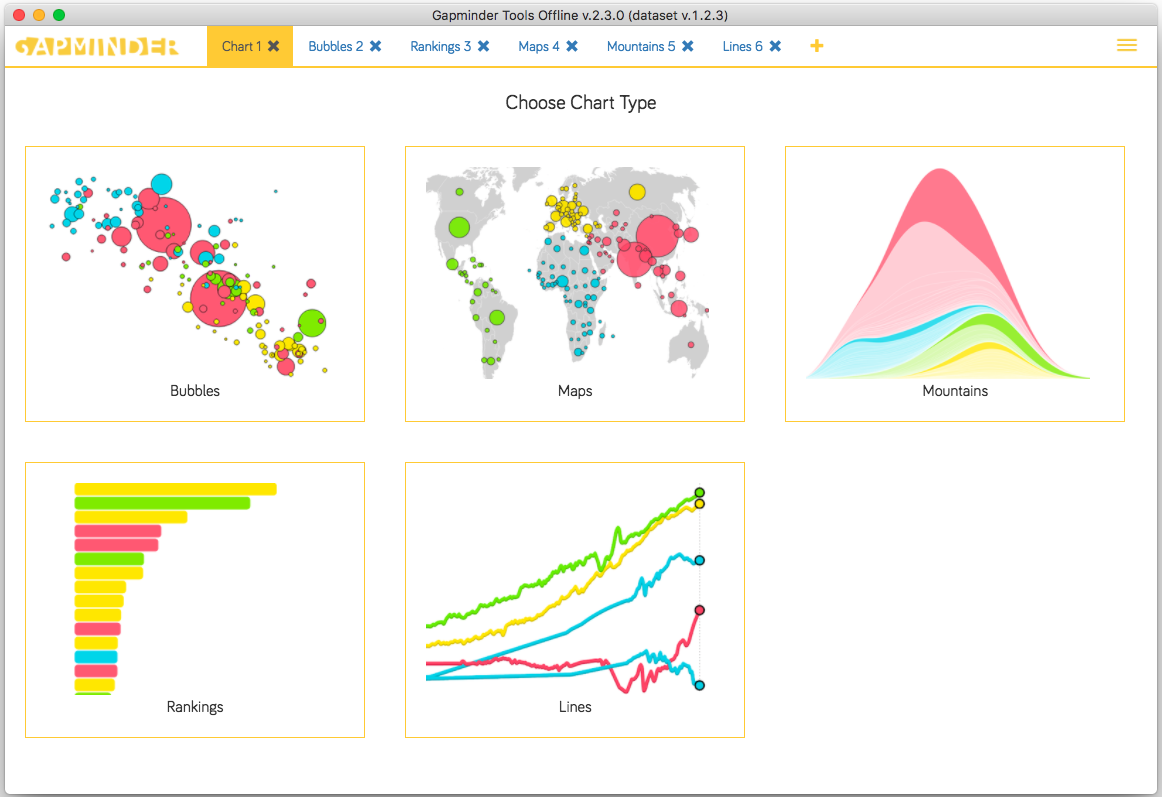
\includegraphics[width=0.95\columnwidth]{figures/home}
	\caption{Gapminder allows to work on multiple visualization at the same time. When creating a new chart, the user is asked to select the wanted type among the $5$ available.}
	\label{fig:home}
\end{figure}

\paragraph{Navigation}
Gapminder allows the user to create and use multiple charts at the same time: each chart is visualized as a tab in the navigation bar.
The navigation bar is located in the top part of the windows and is always visible.
The user can change the chart currently visualized by clicking the corresponding tab in the navigation bar.
To create a new chart, the user can use the \texttt{+} plus button at the end of the navigation bar.
When the user clicks the plus button, a new tab is created and displayed (\cref{fig:home}):
the user can choose a type of chart by clicking the correspondent button.

\paragraph{Right Panel}
The panel on the right contains different controls.
We will describe them from the top to the bottom.
At the very top, a menu allows the user to change the variable encoded as color.
Immediately below, Gapminder shows a colormap for the chosen variable.
Next we find a list of checkbox, one for each country.
This is a filter: it allows the user to select or deselect the countries to show.
At the very bottom there are some buttons that allows to control the zoom level, change the settings or activate the presentation mode.
Depending on the type of chart, Gapminder shows additional buttons in this area;
we will discuss this aspect in the sections about each chart's type.

\paragraph{Chart}
In the center-left part of the screen there is the current chart.
The chart occupies most of the area available on the screen.

\paragraph{Bottom Slider}
In the bottom part of the screen we find a ``play'' button and a time slider.
The button is used to start and stop the animation.
The slider allows to manually change the visualized year.

% TODO... add stuff here?


\subsubsection{Bubbles}
Gapminder's ``bubbles'' is a bubble chart with animations.
We consider the particular instance of bubble chart with the income on the x-axis, the life expectation on the y-axis and the population size encoded as the bubbles size; this is the default visualization offered by Gapminder when creating a new chart of type ``bubbles''.

\begin{figure}[h]
	\centering
	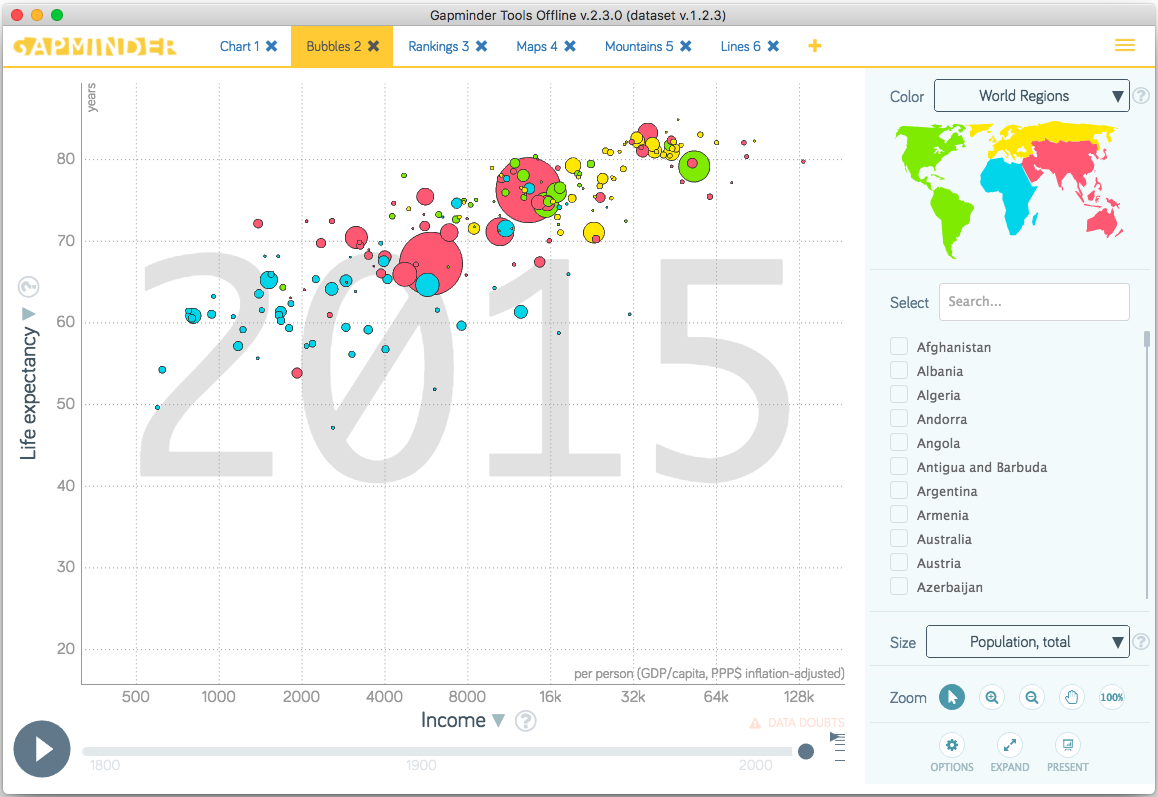
\includegraphics[width=0.95\columnwidth]{figures/bubbles}
	\caption{Chart of type ``bubbles'' in Gapminder.}
	\label{fig:bubbles}
\end{figure}

The visual variables being used are: position, size, color, text labels and animations.


\paragraph{Position}
The position is used to encode the value of $2$ indicators: the position along the x-axis encodes the first indicator (in our case the income), the position along the y-axis the second one (in our case the life expectation).
Since both indicators are quantitative, each point in the chart is in a bijective relation with a pair of possible values for the indicators.

Each point in the bubble chart represents a country.
The encoding is very good, since it uses a single visual variable to represent $2$ dimensions of the dataset.
Position is a very powerful visual variable: it is associative, selective, ordinal and quantitative.
The user will thus:
\begin{itemize}
    \item Perceive each point independently of the other visual variables used. This allows to use other variables (eg. size or color) to encode additional dimensions of the data.
    \item Perceive each point as different from each other. This allows to easily distinguish countries from each other on the chart.
    \item Be able to easily order the points. This allows to easily tell which countries have lowest and highest values for one indicator and order the countries based on some indicator.
    \item Be able to easily compute ratios between the values of the indicators encoded by each point. This allows to compare the situation of pairs of different countries from the point of view of the $2$ indicator.
\end{itemize}

Additionally, the position visual variable is used in the colormap for the world's regions, as explained in colors paragraph.
% TODO: we can force the tool to use categorical data for x-axis / y-axis !!! BAD
% Nevertheless, Gapminder allows the user to select other kinds of attributes as well, which might lead to sub-optimal representations.


\paragraph{Size}
The size is used to encode the third indicator, in our case the population size.
In particular, the value is encoded as the area of the bubble.

Size is selective, ordinal and quantitative.
The user can thus:
\begin{itemize}
    \item Easily perceive countries with different populations as different from each other.
    \item Easily order countries by population size.
    \item Easily compute ratios between the size of the populations of different countries.
\end{itemize}

However, the tool does not visualize a legend for the sizes of the bubble.
This makes difficult to perform the inverse mapping from area of the bubble to size of the population by just looking at the bubble chart.
The value is visualized on the right side of the screen only if the user moves the mouse over a bubble.

The encoding of the population sizes is overall clear, but it can be improved.
On the one hand, the user is able to distinguish and compare the population of different countries.
On the other hand, it is quite complex to visualize the real values of the populations.


\paragraph{Color}
\label{paragraph:bubbles-color}
The color can be used to encode any of the available dimensions of the dataset.
In our case, the tool uses the color to encode the world region to which each country belongs.
Gapminder shows a colormap in the top right corner of the windows:
the colormap is visualized a small stylized planisphere where each continent if filled with the color that corresponds to its region.
The tool differentiate $4$ world regions: americas, africa, europe and russia, asia and oceania.

The colormap is categorical and uses different color hues for each different value.
The visualization uses the following $4$ colors: green, blue, yellow, red.
The choice of the color is good, since they are all distinct.
There is no way to change the colormap or force a different mapping.
However it does not take into account colorblind people that might have difficulties in distinguish green and red.

Each bubble has a black border.
This makes it easier to identify a bubble and distinguish it from the other ones.

The color of a bubble together with the colormap allows to match each country with a specific location on the planisphere.
In other words, this allows the user to approximately locate the geographical position of each county.

The encoding if clear: the $4$ choses colors are very different from each other, so it is very easy to distinguish point that corresponds to countries in different regions.
The inverse mapping from color to region of the world is also pretty straightforward, since there are only $4$ possible regions.

The visualization uses a white background, with a big gray text label in the center (to visualize the year, see the animation paragraph).
This is a good design choice, since it is a neutral color that does not interfere with the visualization and creates a high contrast with the colors used for the bubbles.

%, but it is possible to select any other attribute.
% The tool automatically recognize the type of the attribute and uses an appropriate encoding.
% In case of categorical data, the tool generates a legend for the colors: each color is associated with a different categorical values.
% In case of qualitative data, the tool generates a continuos rainbow colormap, ranging from violet to represent the minimum value to red that to represent the maximum.
% It is possible to choose between the linear or a logarithmic scale using the dedicated menu;
% by default the tool uses a linear scale.

\paragraph{Text Labels}
Text labels are used to show the name of the indicator visualized on the axises, the measure units and the value for the ticks.
The measure unit is shown above to the right for the x-axis.
Below the axis there are the values for the ticks (about $10$).
Below them in the center there is the name of the indicator.
All labels are gray.
The y-axis is similar.

% TODO: describe better

Labels are used to visualize additional information about the bubbles.
When the user selects a particular bubble (either by moving the mouse over it or selecting the checkbox of the corresponding country in the right panel), a text label is shown to the top right of the bubble.
The text label contains the name of the country, followed by the year.

Additionally, $2$ dashed lines parallel to the axis are displayed when the mouse pointer is over a bubble.
The lines start to from the bubble and intercept respectively the x and y-axis.
A new text label with the value for the indicators of the country that corresponds to the bubble is shown at the intersection with the axis.
This is a good design choice, since it allows the user to easily obtain additional information about interesting countries without polluting the visualization with the details about all the countries.

\paragraph{Animation}
TODO...

\subsubsection{Maps}

\subsubsection{Mountains}

\subsubsection{Rankings}

\subsubsection{Lines}


\subsection{Improvements}
TODO...
Bullet list of points to discuss:
\begin{itemize}
    \item add a legend for the size of the bubbles
    \item add information about the 3 indicators in the tooltip of the bubble (proximity gestalt law)

    \item colormap... not easy to read for colorblind people... possibility to choose a different colormap for colorblind people, since there are only 4 colors
\end{itemize}
